% ==============================================
% ELEMENTOS PÓS-TEXTUAIS
% ==============================================
\postextual

% ||||||||||||||||||||||||||||||||||||||||||||||
% REFERÊNCIAS BIBLIOGRÁFICAS
% ||||||||||||||||||||||||||||||||||||||||||||||
\bibliography{references}

% ----------------------------------------------
% Glossário
% ----------------------------------------------
% Consulte o manual da classe abntex2 para orientações sobre o glossário.
%
%\glossary

% ||||||||||||||||||||||||||||||||||||||||||||||
% APÊNDICES
% ||||||||||||||||||||||||||||||||||||||||||||||
\begin{apendicesenv}

\partapendices

% ----------------------------------------------
% Apêndice 1
% ----------------------------------------------
\chapter{CÓDIGO NO PYTHON}

\begin{figure}[!htb]
\centering
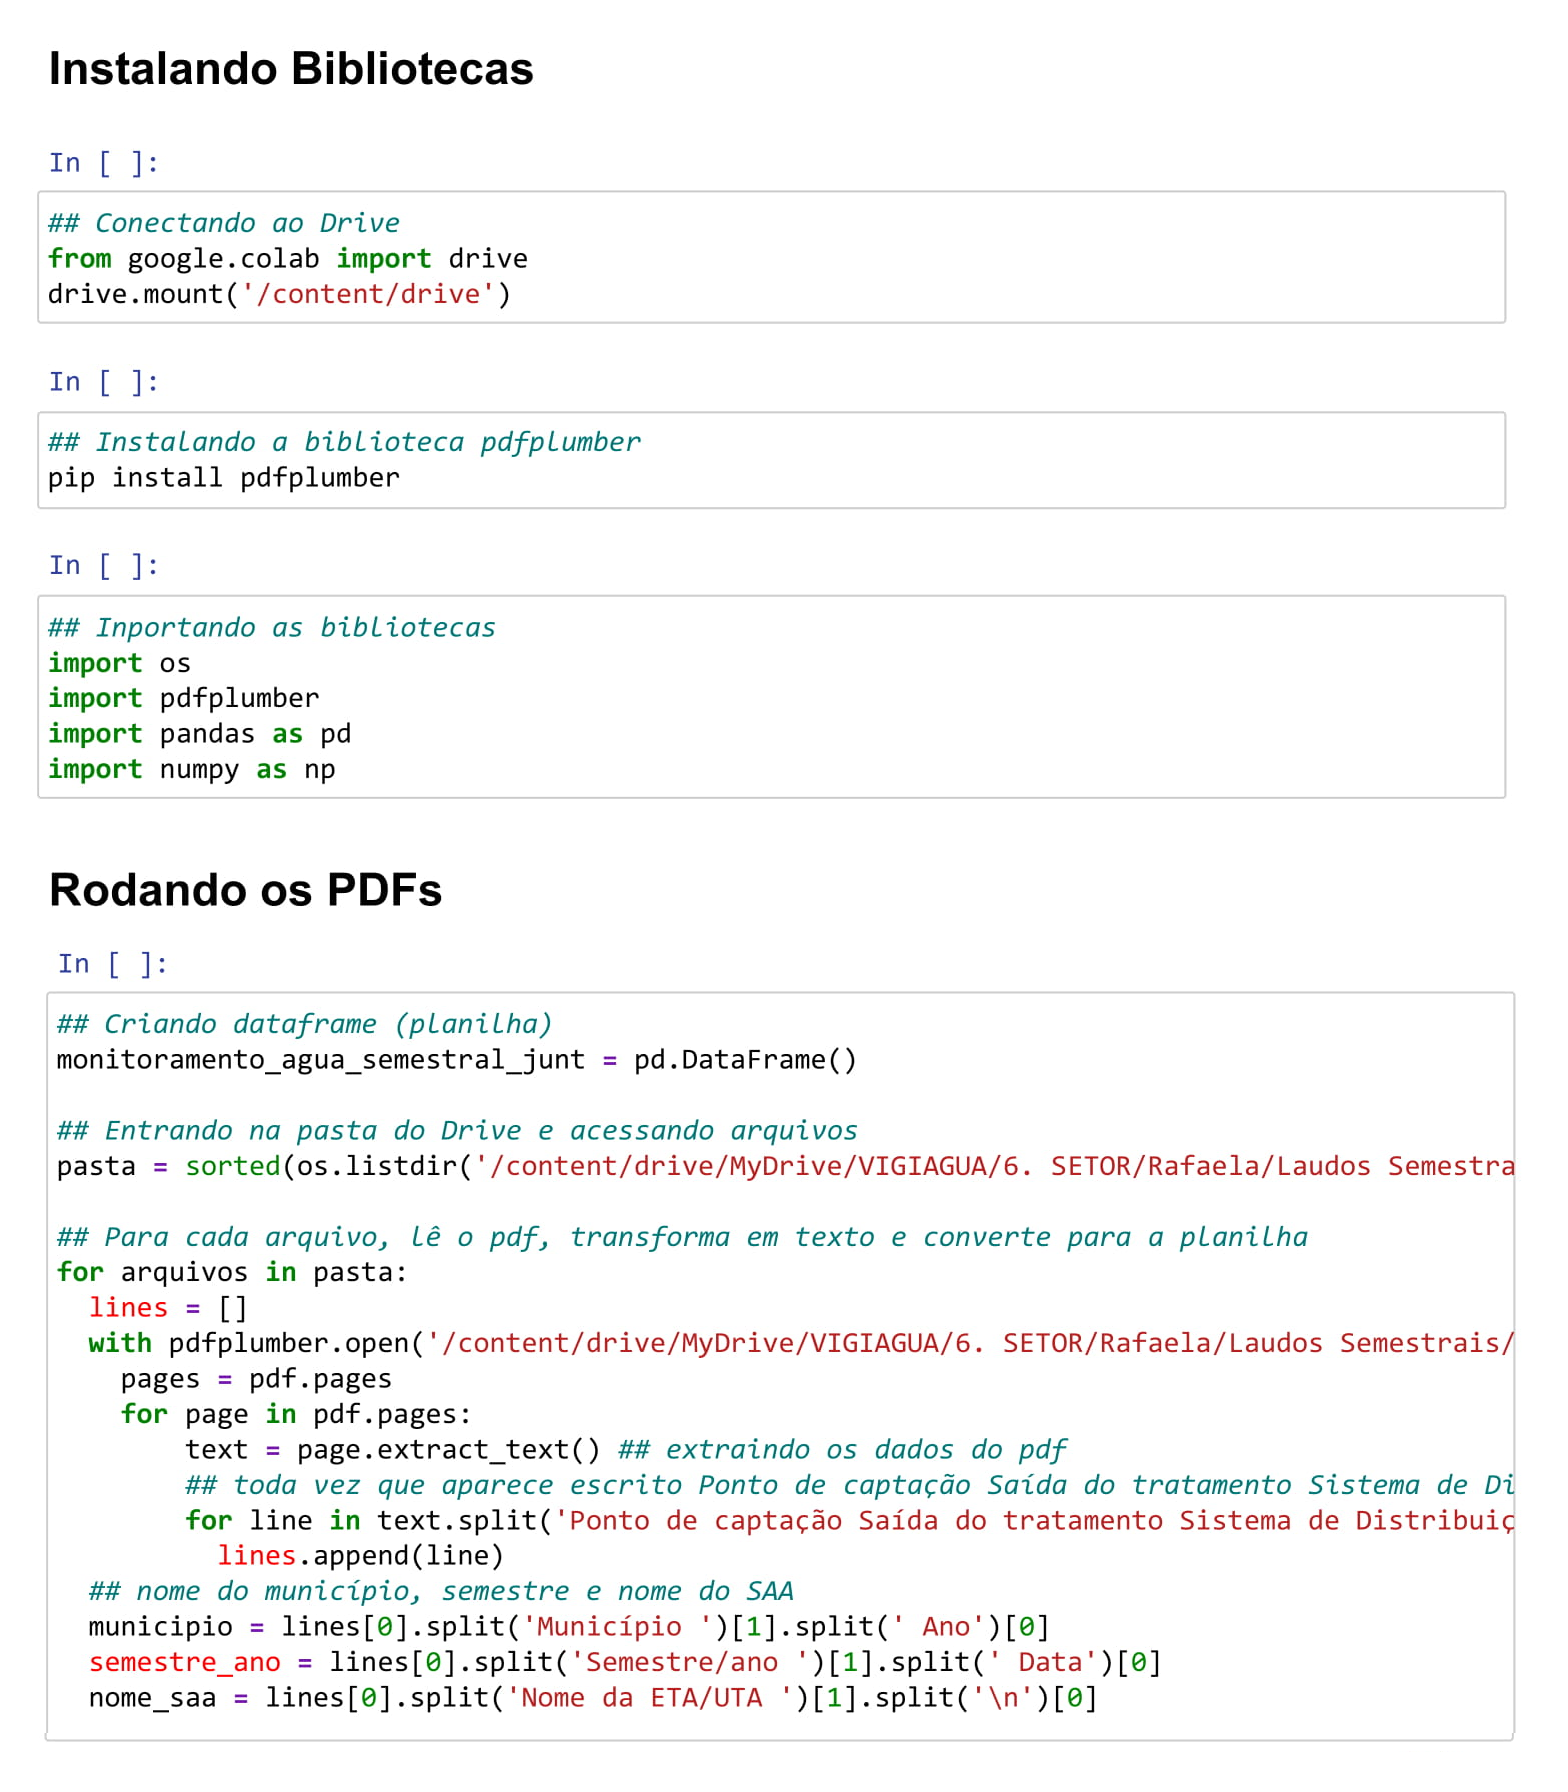
\includegraphics[scale=0.4]{colab/laudos 1.png}
\label{fig04}
\end{figure}

\begin{figure}[!htb]
\centering
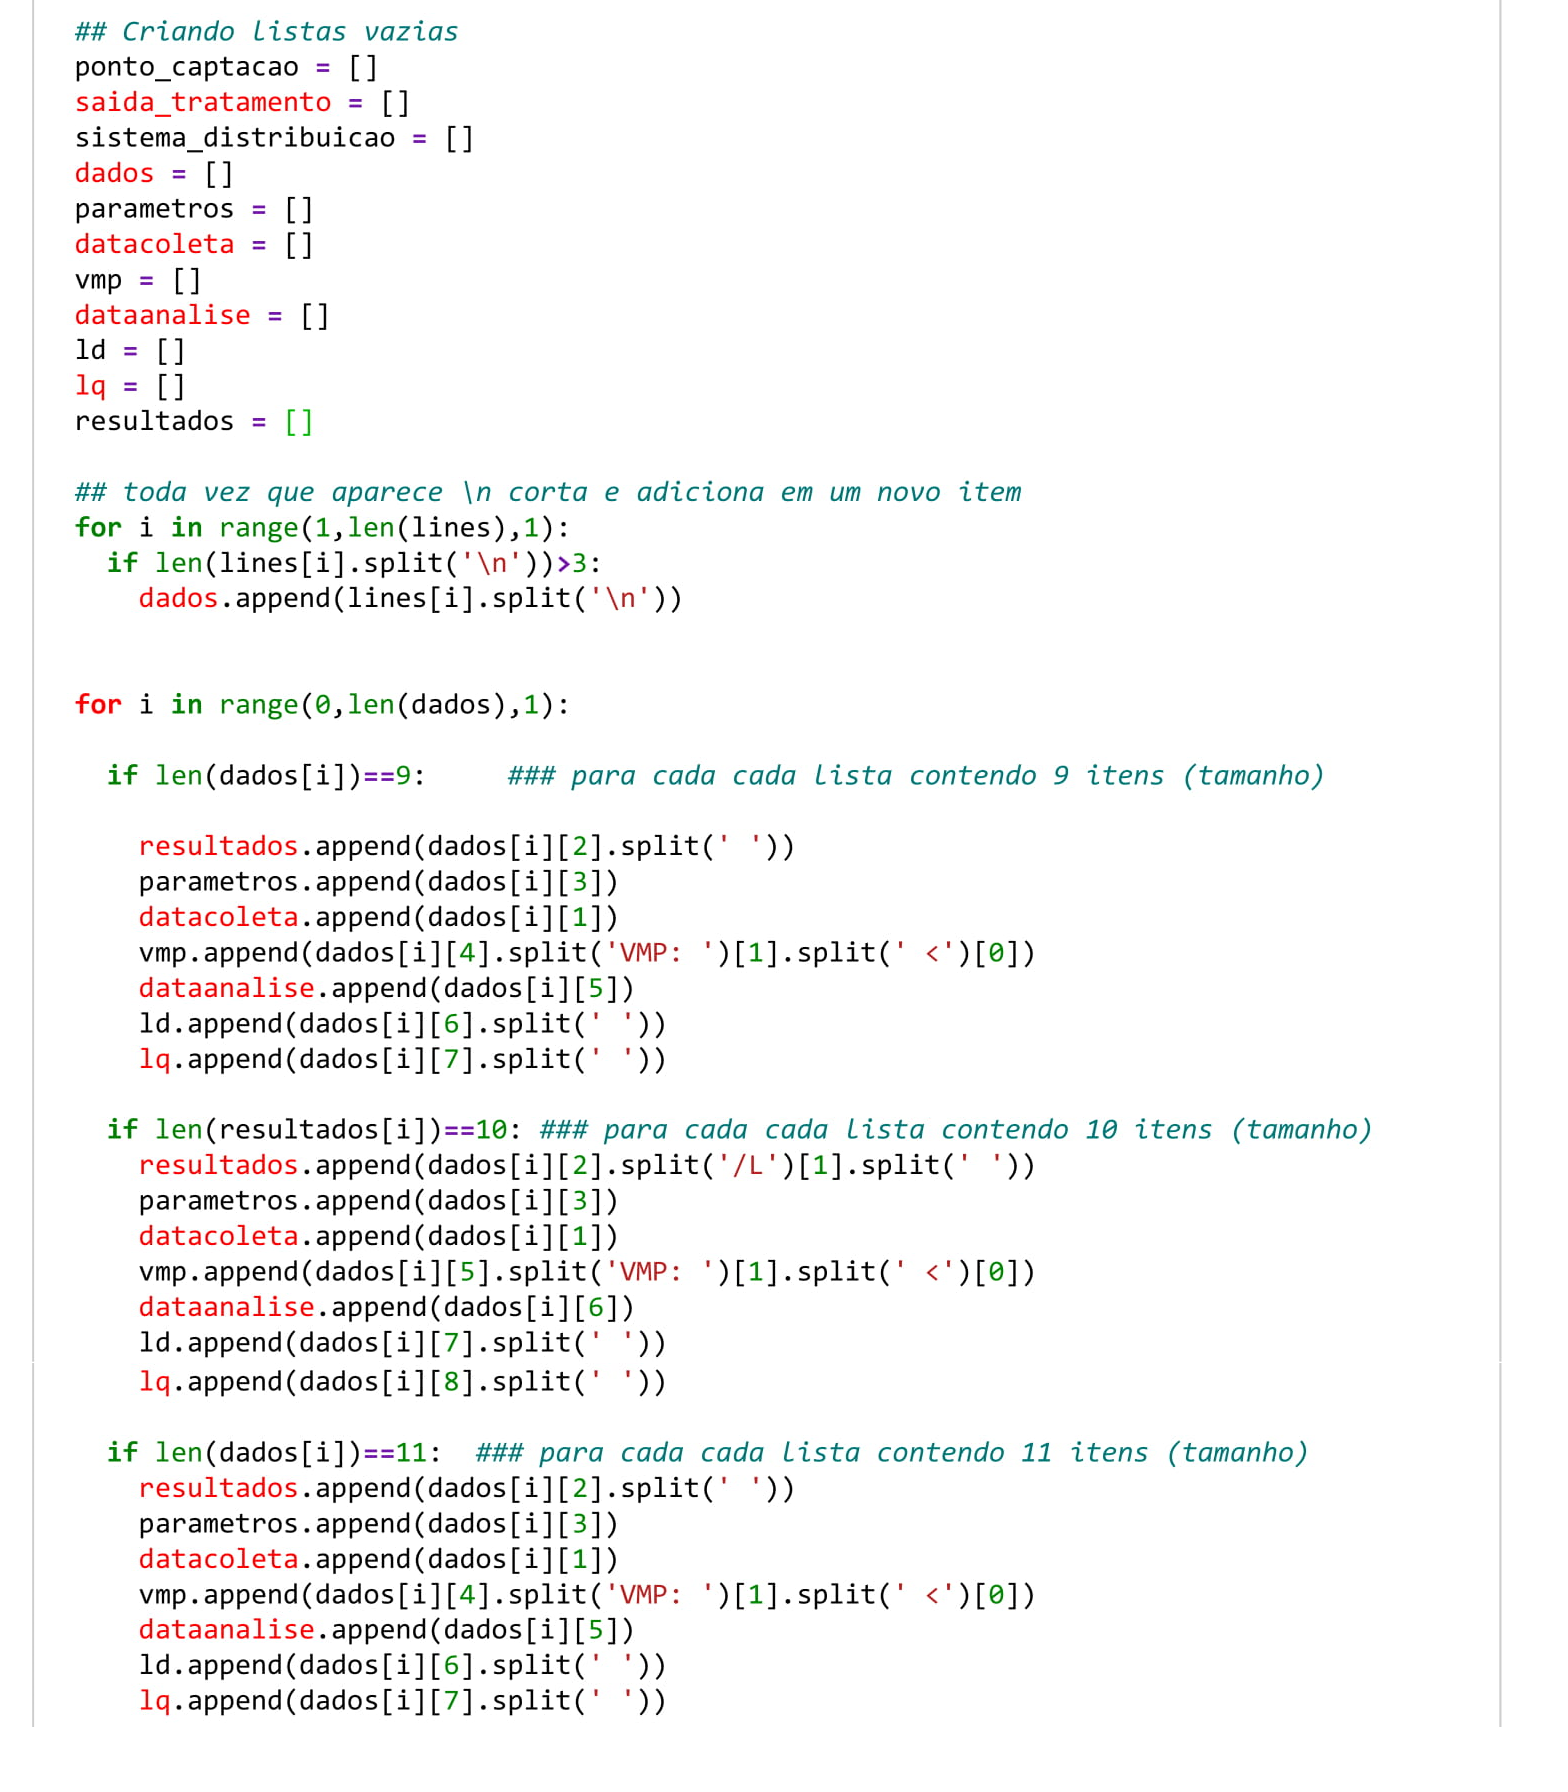
\includegraphics[scale=0.4]{colab/laudos 2.png}
\label{fig04}
\end{figure}

\begin{figure}[!htb]
\centering
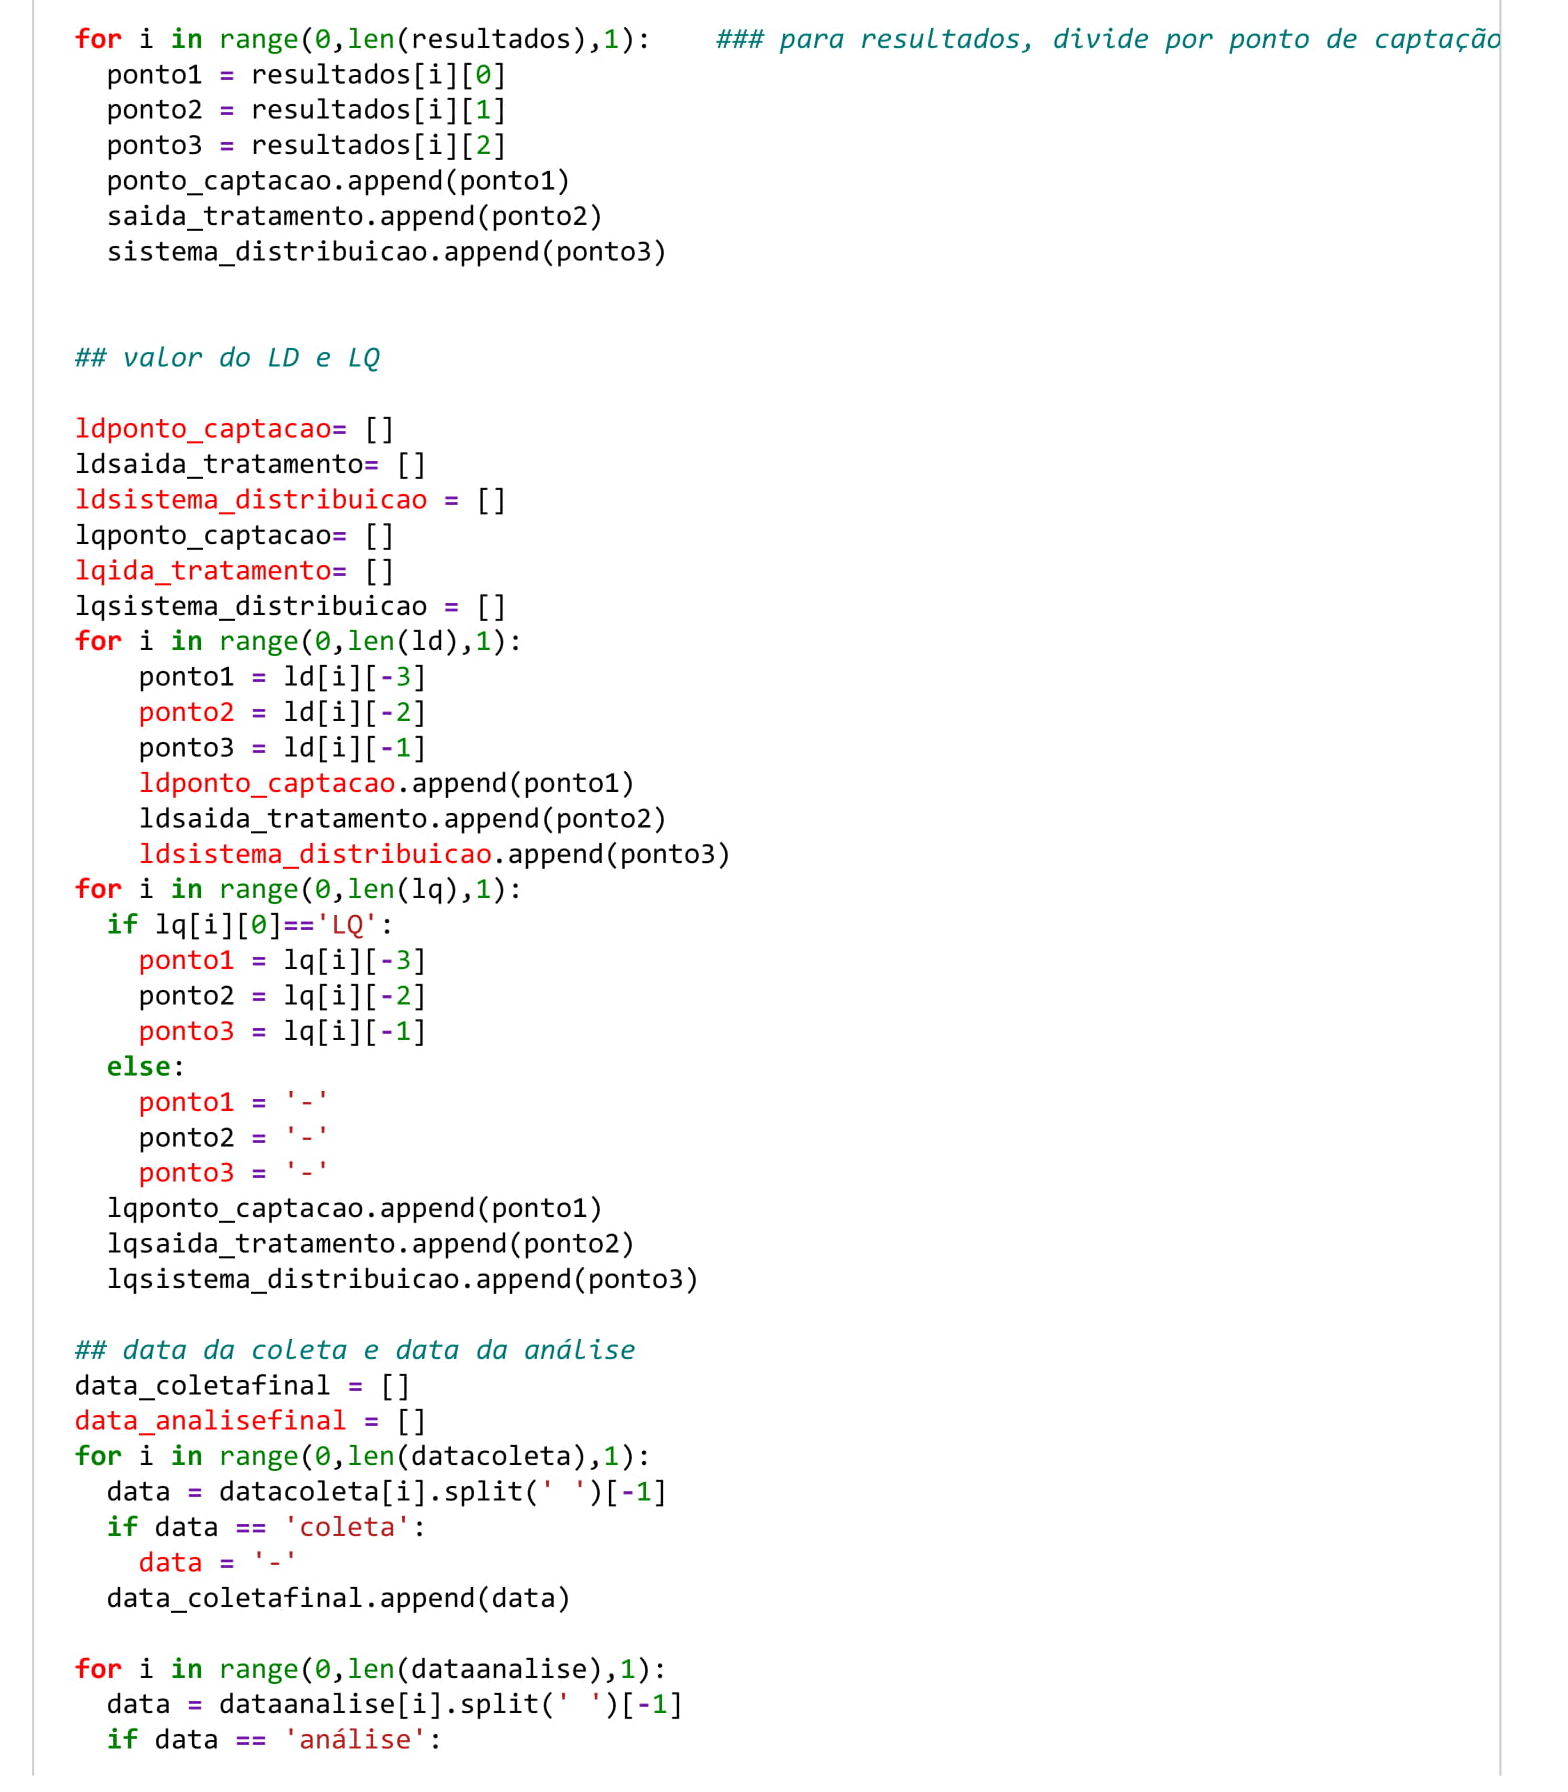
\includegraphics[scale=0.4]{colab/laudos 3.png}
\label{fig04}
\end{figure}

\begin{figure}[!htb]
\centering
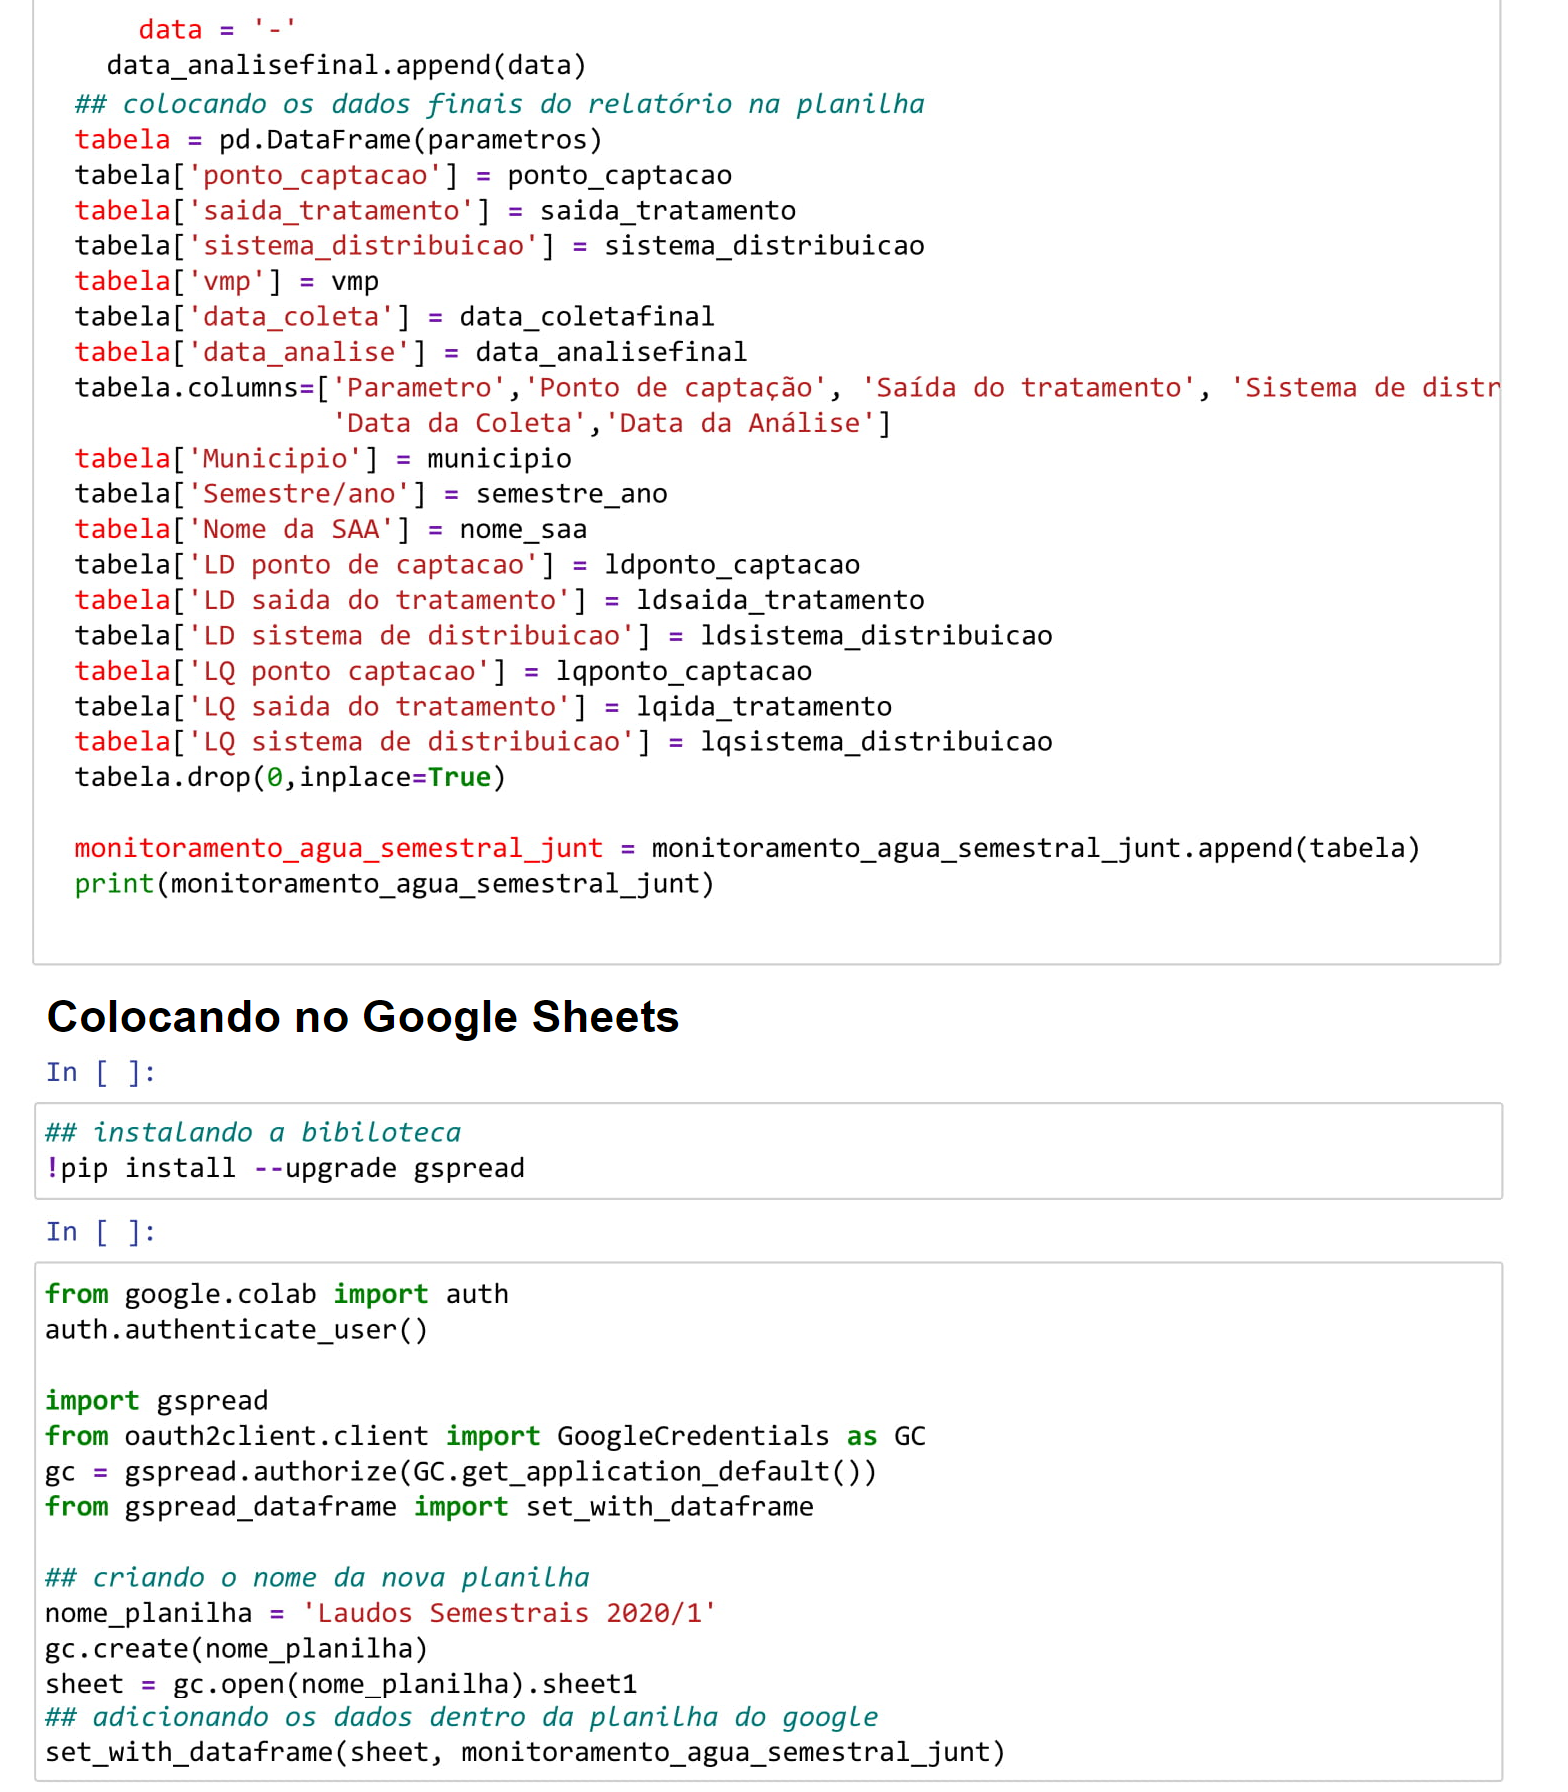
\includegraphics[scale=0.4]{colab/laudos 4.png}
\label{fig04}
\end{figure}

% ----------------------------------------------
% Apêndice 2
% ----------------------------------------------
\chapter{Municípios que Não Possuem Resultados de THMs}

\begin{table}[!htb]
\centering
\footnotesize
\label{tab:com_esp}
    \begin{tabular}{lcc}
    \toprule
    \textbf{Município} & \textbf{Manancial} & \textbf{População Abastecida} \\ \hline
      Alto Feliz              & Subterrâneo        & 2.910                         \\
Anta Gorda              & Subterrâneo        & 4.188                         \\
Arroio do Padre         & Subterrâneo        & 1.386                         \\
Bom Princípio           & Subterrâneo        & 8.048                         \\
Candiota                & Superficial        & 7.843                         \\
Canudos do Vale         & Subterrâneo        & 485                           \\
Capão do Cipó           & Subterrâneo        & 1.444                         \\
Capitão                 & Subterrâneo        & 2.729                         \\
Cerro Branco            & Subterrâneo        & 764                           \\
Dois Lajeados           & Subterrâneo        & 1.683                         \\
Estrela Velha           & Subterrâneo        & 1.314                         \\
Forquetinha             & Subterrâneo        & 1.896                         \\
Gramado Xavier          & Subterrâneo        & 1.959                         \\
Guabiju                 & Subterrâneo        & 1.060                         \\
Herveiras               & Subterrâneo        & 1.968                         \\
Hulha Negra             & Subterrâneo        & 3.317                         \\
Ibarama                 & Subterrâneo        & 1.576                         \\
Imigrante               & Subterrâneo        & 1.984                         \\
Inhacorá                & Subterrâneo        & 1.449                         \\
Itacurubi               & Subterrâneo        & 1.358                         \\
Ivoti                   & Subterrâneo        & 20.720                        \\
Jari                    & Subterrâneo        & 1.047                         \\
Monte Alegre dos Campos & Subterrâneo        & 1.396                         \\
Muçum                   & Subterrâneo        & 4.862                         \\
Nova Pádua              & Subterrâneo        & 1.306                         \\
Novo Cabrais            & Subterrâneo        & 937                           \\
Paraíso do Sul          & Superficial        & 3.850                         \\
Passo do Sobrado        & Subterrâneo        & 5.109                         \\
Picada Café             & Subterrâneo        & 5.625                         \\
Pinhal da Serra         & Subterrâneo        & 432                           \\
Pinhal Grande           & Subterrâneo        & 774                           \\
Progresso               & Subterrâneo        & 3.060                         \\
Protásio Alves          & Subterrâneo        & 628                           \\
Quevedos                & Subterrâneo        & 1.640                         \\
Relvado                 & Subterrâneo        & 1.663                         \\
São Martinho da Serra   & Subterrâneo        & 2.129                         \\
São Valentim do Sul     & Subterrâneo        & 2.080                         \\
São Vendelino           & Subterrâneo        & 2.243                         \\
Segredo                 & Subterrâneo        & 2.827                         \\
Sério                   & Subterrâneo        & 891                           \\
Sinimbu                 & Subterrâneo        & 5.681                         \\
Toropi                  & Subterrâneo        & 945                           \\
Turuçu                  & Superficial        & 3.113                         \\
Vale Real               & Subterrâneo        & 5.698                         \\
Vespasiano Corea        & Subterrâneo        & 727                           \\
Westfalia               & Subterrâneo        & 3.007                         \\\hline
\multicolumn{2}{c}{\textbf{Total}}           & \textbf{131.751}              \\ \bottomrule
    \end{tabular}
    
    \label{tab01}
\end{table}




\end{apendicesenv}

% ||||||||||||||||||||||||||||||||||||||||||||||
% ANEXOS
% ||||||||||||||||||||||||||||||||||||||||||||||
%\begin{anexosenv}
% Imprime uma página indicando o início dos anexos
%\partanexos

% ----------------------------------------------
% Anexo 1
% ----------------------------------------------
%\chapter{Datasheet}\label{anexo1}
%\includepdf[pages=-]{pdfs/Datasheet.pdf}

% ----------------------------------------------
% Anexo 2
% ----------------------------------------------
%\chapter{Anexo 2}

%\end{anexosenv}

% ==============================================
% INDICE REMISSIVO
% ==============================================
\phantompart
\printindex
% ----------------------------------------------


